\documentclass[conference]{IEEEtran}
\IEEEoverridecommandlockouts
% The preceding line is only needed to identify funding in the first footnote. If that is unneeded, please comment it out.
\usepackage{cite}
\usepackage{amsmath,amssymb,amsfonts}
%\usepackage{algorithmic}
\usepackage{graphicx}
\usepackage{textcomp}
\usepackage{xcolor}
\def\BibTeX{{\rm B\kern-.05em{\sc i\kern-.025em b}\kern-.08em
    T\kern-.1667em\lower.7ex\hbox{E}\kern-.125emX}}

%%%%%%%%%%%%%%%%%%%%%%%%%%%%%%%%%%%%%%%%%%%%%%%%%%%%%%%%%%%%%%%%%%%%%%%%%%%%%%%%%%%%%%%

\newenvironment{note}{
	\color{gray}
}

%%%%%%%%%%%%%%%%%%%%%%%%%%%%%%%%%%%%%%%%%%%%%%%%%%%%%%%%%%%%%%%%%%%%%%%%%%%%%%%%%%%%%%%


\begin{document}

\title{\huge{Métodos de \textit{Deep Learning} aplicados à Segmentação Semântica de Imagens para Percepção de Veículos Autônomos}}

\author{\IEEEauthorblockN{Gabriel Toffanetto França da Rocha}
\IEEEauthorblockA{\textit{Laboratório de Mobilidade Autônoma -- LMA} \\
\textit{Faculdade de Engenharia Mecânica, Universidade Estadual de Campinas}}\\
Campinas, Brasil \\
g289320@dac.unicamp.br}

\maketitle

\begin{abstract}

\begin{note}
	\begin{itemize}
		\item Veículos autonomos
		\item Visão computacional
		\item Percepção do ambiente
		\item Segmentação Semântica de Imagem
		\item Métodos Vanilla
		\item Métodos Deep Learning
		\item Necessidades da aplicação
		\item Resultados
		\item Proximos passos (teste para obtenção do Perception grid)
	\end{itemize}
\end{note}

\end{abstract}

\begin{IEEEkeywords}
Deep learning, Visão computacional, Segmentação Semântica de Imagem, Robótica móvel, Veículos autônomos
\end{IEEEkeywords}

\section{Introdução} \label{sc:introducao}

%% ToDo

%\begin{note}
%	
%	\begin{itemize}
%		\item Veículos autônomos 
%		\begin{itemize}
%			\item VILMA \cite{garcia2018VILMAIntelligentVehicle}
%		\end{itemize}
%		\item Métodos de navegação 
%		\begin{itemize}
%			\item Segmentação de imagem para mapeamento de área navegável e obstáculos \cite{jebamikyousAutonomousVehiclesPerception2022}
%			\item Citar método do Giovani \cite{vitor2021ModelingEvidentialGrids}
%		\end{itemize}
%		\item Comparar como era feito e como é feito hoje em dia
%		\item Mostrar a ideia vantajosa de utilizar \textit{Deep Learning}  \cite{geron2020HandsonMachineLearning}
%		\begin{itemize}
%			\item Dispensa de pré-processamento
%			\item Robustez à variação de luz, reflexos (desde que esses sejam usados em treinamento) \cite{papadeas2021RealTimeSemanticImage}
%			\item \textit{Datasets} para treinamento \cite{cordts2016CityscapesDatasetSemantic, brostow2008SegmentationRecognitionUsing, brostow2009SemanticObjectClasses, jin2021RaidaRRichAnnotated}
%		\end{itemize}
%	\end{itemize}
%
%
%\end{note}

Veículos com capacidade de se guiarem de forma autônoma estão cada vez mais presentes no dia a dia da sociedade contemporânea, possibilitando que o motorista possa realizar outras atividades durante a navegação, ou que o mesmo seja assistido em caso de alguma falha humana do condutor. Para que o automóvel seja capaz de se mover por conta própria, o mesmo deve ser capaz de perceber o ambiente, e sensores como sonares, radares, LiDARs e câmeras podem ser utilizados para tal. Porém, a câmera se faz como uma solução mais viável economicamente, e como visto na literatura, apresenta soluções que contemplam os desafios da navegação autônoma de veículos em ambientes urbanos, como visto nos trabalhos de \cite{garcia2018VILMAIntelligentVehicle} e \cite{vitor2014UrbanEnvironmentNavigation}.

Para que um veículo autônomo possa entender o ambiente à sua volta, é necessário que ele saiba reconhecer as entidades que o compõem, como por exemplo: estrada, veículos, calçadas, pedestres e vegetação, para que assim, o mesmo saiba diferenciar área navegável de obstáculos \cite{jebamikyousAutonomousVehiclesPerception2022}. Para isso, o emprego da técnica de segmentação semântica de imagens, onde cada pixel da imagem é classificado de acordo com a entidade do ambiente da qual ele faz parte \cite{he2016ImageSegmentationTechniques}. A Fig.~\ref{fig:dynamiclocalperception} mostra a aplicação da técnica de segmentação semântica fundida à informação de profundidade dada por uma câmera \textit{stereo}, permitindo a obtenção de um \textit{grid} de percepção dinâmica local (DLP), que projeta no plano 2D o ambiente contendo a detecção de múltiplos objetos para que o veículo consiga planejar seu caminho \cite{vitor2021ModelingEvidentialGrids}.

\begin{figure}[h!]
	\centering
	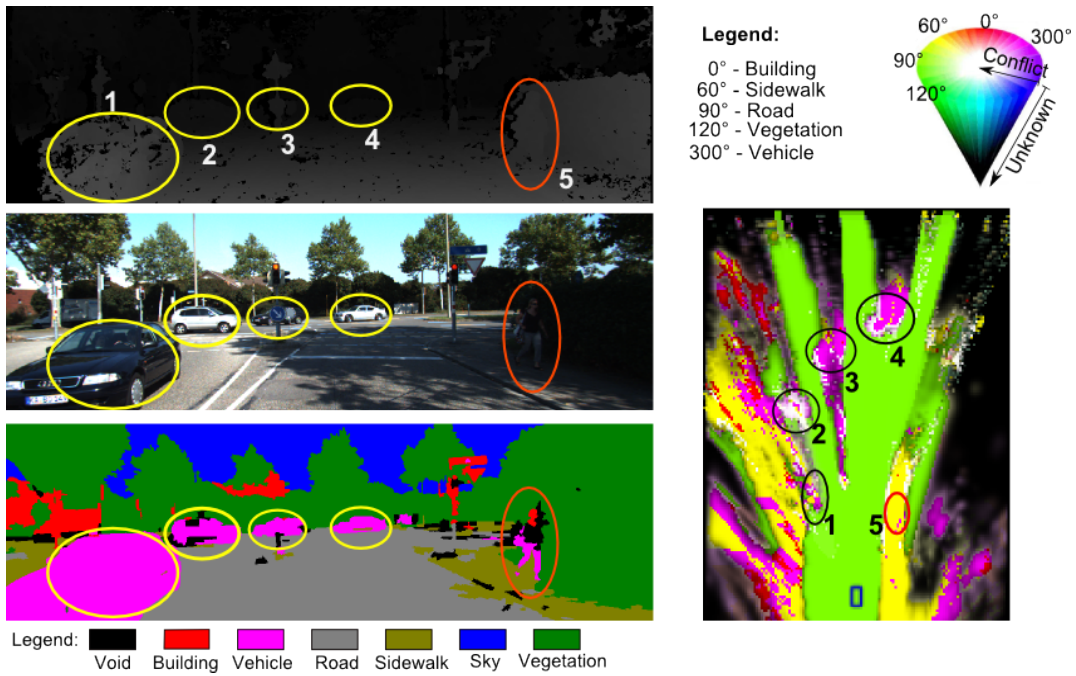
\includegraphics[width=\linewidth]{img/dynamic_local_perception}
	\caption{DLP com ênfase na detecção múltipla de objetos móveis obtido com a fusão da imagem semanticamente segmentada e as informações de profundidade \cite{vitor2021ModelingEvidentialGrids}.}
	\label{fig:dynamiclocalperception}
\end{figure}

Existem métodos de processamento de imagens que realizam o mascaramento de cada entidade da imagem, porém a definição de qual é a classe de cada segmento se faz desafiadora, sendo anteriormente empregada a utilização de redes neurais artificiais (ANNs) para tal, como feito por \cite{vitor20132D3DVision}. Porém, devido à utilização de ANNs somente para a classificação final, era necessário muito pré-processamento para realização da segmentação semântica. Com o desenvolvimento das redes neurais profundas (DNNs), obteve-se métodos com poder suficiente para que, dada uma imagem bruta de entrada e uma imagem de referência (\textit{ground truth}) segmentada para comparação, a rede profunda consegue aprender como realizar a segmentação da imagem do ambiente urbano, como nas várias arquiteturas mostradas por \cite{papadeas2021RealTimeSemanticImage}. Com a popularização desses métodos, já existem diversos conjuntos de dados para treinamento das DNNs, como os \cite{cordts2016CityscapesDatasetSemantic} e \cite{brostow2008SegmentationRecognitionUsing,brostow2009SemanticObjectClasses}. Existem também \textit{datasets} que trazem cenas ainda mais desafiadoras, como o \cite{jin2021RaidaRRichAnnotated} que apresenta imagens urbanas durante noites chuvosas.

Dessa forma, a percepção do ambiente por meio de visão computacional se faz indispensável para o desenvolvimento dos veículos autônomos, e com isso, os métodos de \textit{deep learning} se fazem uma grande ferramenta para conseguir-se reconhecer as entidades de uma cena urbana com robustez às variações de luz e reflexos, sendo assim uma solução a ser explorada. Além do desempenho da segmentação semântica, o tempo demandado para tal operação também é vital, uma vez que durante a navegação, todos os módulos operam em tempo real, e a quantidade de \textit{frames} segmentados por segundo é uma informação importante. Dessa forma, esse trabalho propõem a utilização de redes neurais profundas com diferentes arquiteturas para a segmentação semântica de imagens de cenas urbanas, utilizados \textit{datasets} da literatura e para testes finais, utilizando imagens reais adquiridas pelo autor.

Este trabalho é dividido em seis partes, onde na Seção~\ref{sc:introducao} é realizada a motivação e contextualização da pesquisa e na Seção~\ref{sc:estado-da-arte} é apresentado o estado da arte, discorrendo sobre as soluções utilizadas atualmente. Com isso, a Seção~\ref{sc:metodologia} apresenta a metodologia a ser utilizada neste trabalho, seguida dos resultados obtidos na Seção~\ref{sc:resultados} e sua análise na Seção~\ref{sc:analise}. Por fim, são apresentadas as conclusões na Seção~\ref{sc:conclusoes} e as referências utilizadas.


\section{Estado da arte} \label{sc:estado-da-arte}



\begin{note}
	\begin{itemize}
		\item Estratégias para operação em real time
		\item Artigos \textit{Survey} \cite{janai2020ComputerVisionAutonomous}
		\item Tipos de redes utilizadas \cite{chao2019HarDNetLowMemory,fan2021RethinkingBiSeNetRealtime, wang2019ESNetEfficientSymmetric, yu2020BiSeNetV2Bilateral, yu2018BiSeNetBilateralSegmentation,poudel2018ContextNetExploringContext,badrinarayanan2016SegNetDeepConvolutional} 
		\item Resultados estado-da-arte \cite{papadeas2021RealTimeSemanticImage}
		\begin{itemize}
			\item mIoU
			\item FPS
		\end{itemize}
	\end{itemize}
\end{note}


\section{Metodologia} \label{sc:metodologia}

\begin{note}
	\begin{itemize}
		\item Arquiteturas escolhidas 
		\item Redes escolhidas
		\item \textit{Datasets} escolhidos
		\begin{itemize}
			\item Proposta de utilizar dados coletados no \textit{campus}
		\end{itemize}
		\item Método de treinamento
		\item Métricas utilizadas
		\item \textit{Frameworks} utilizados
		\item \textit{Hardware} utilizado
		
	\end{itemize}
\end{note}

Para a solução do problema foi escolhida a rede STDC1-50, que apresentou maior velocidade nos testes realizados pelos autores do \textit{survey} \cite{papadeas2021RealTimeSemanticImage}, com um desempenho de segmentação considerável. [...]

\subsection{Arquitetura}

A rede STDC1 \cite{fan2021RethinkingBiSeNetRealtime} é baseada na arquitetura de \textit{two-branch network}, onde existe uma bifurcação da rede em dois ramos, um ligado à extração de informações de contexto e o outro aplicado para obtenção de informações espaciais da entrada. A informação de contexto demanda de uma maior profundidade, implementando mecanismos de atenção em dois níveis para extração dos atributos necessários para a identificação das regiões da imagem, como mostrado na Fig.~\ref{fig:stdcseg-architecture}(a).

Porém, o fato de se processar a informação de entrada em dois ramos, traz um inconveniente para o problema de segmentação em tempo real, que é justamente o tempo de inferência da rede. Desta forma, a rede aplica uma estratégia elegante ao utilizar no lugar de um ramo com novas camadas, uma \textit{skip connection} do \textit{Stage 3}, para o bloco de fusão [...]. Para forçar a captura das informações espaciais, a saída da \textit{skip connection} é utilizada em uma tarefa auxiliar de detecção de bordas de cada região semântica da imagem, por meio de uma \textit{detail head}. Tal procedimento é realizado por meio de treinamento supervisionado, onde com a aplicação de filtros laplacianos na imagem rótulo de segmentação semântica, se obtém a imagem rótulo com as bordas de cada segmento da imagem de entrada, que representam os detalhes à serem capturados pelo ramo espacial, e a perda é computada por meio da saída da \textit{detail head} e o rótulo obtido. Reforça-se que esse procedimento é realizado apenas em treinamento, enquanto durante a inferência a rede neural irá utilizar as habilidades aprendidas por meio do gradiente sobre a perda atrelada à segmentação e à detecção de bordas, sem realizar explicitamente a extração das bordas de cada região da imagem.

Cada estágio é composto da forma ... E realiza convolução da forma...

O mecanismo de atenção é ...

Por fim, a fusão é feita ... e o upsampling...

\begin{figure}[h!]
	\centering
	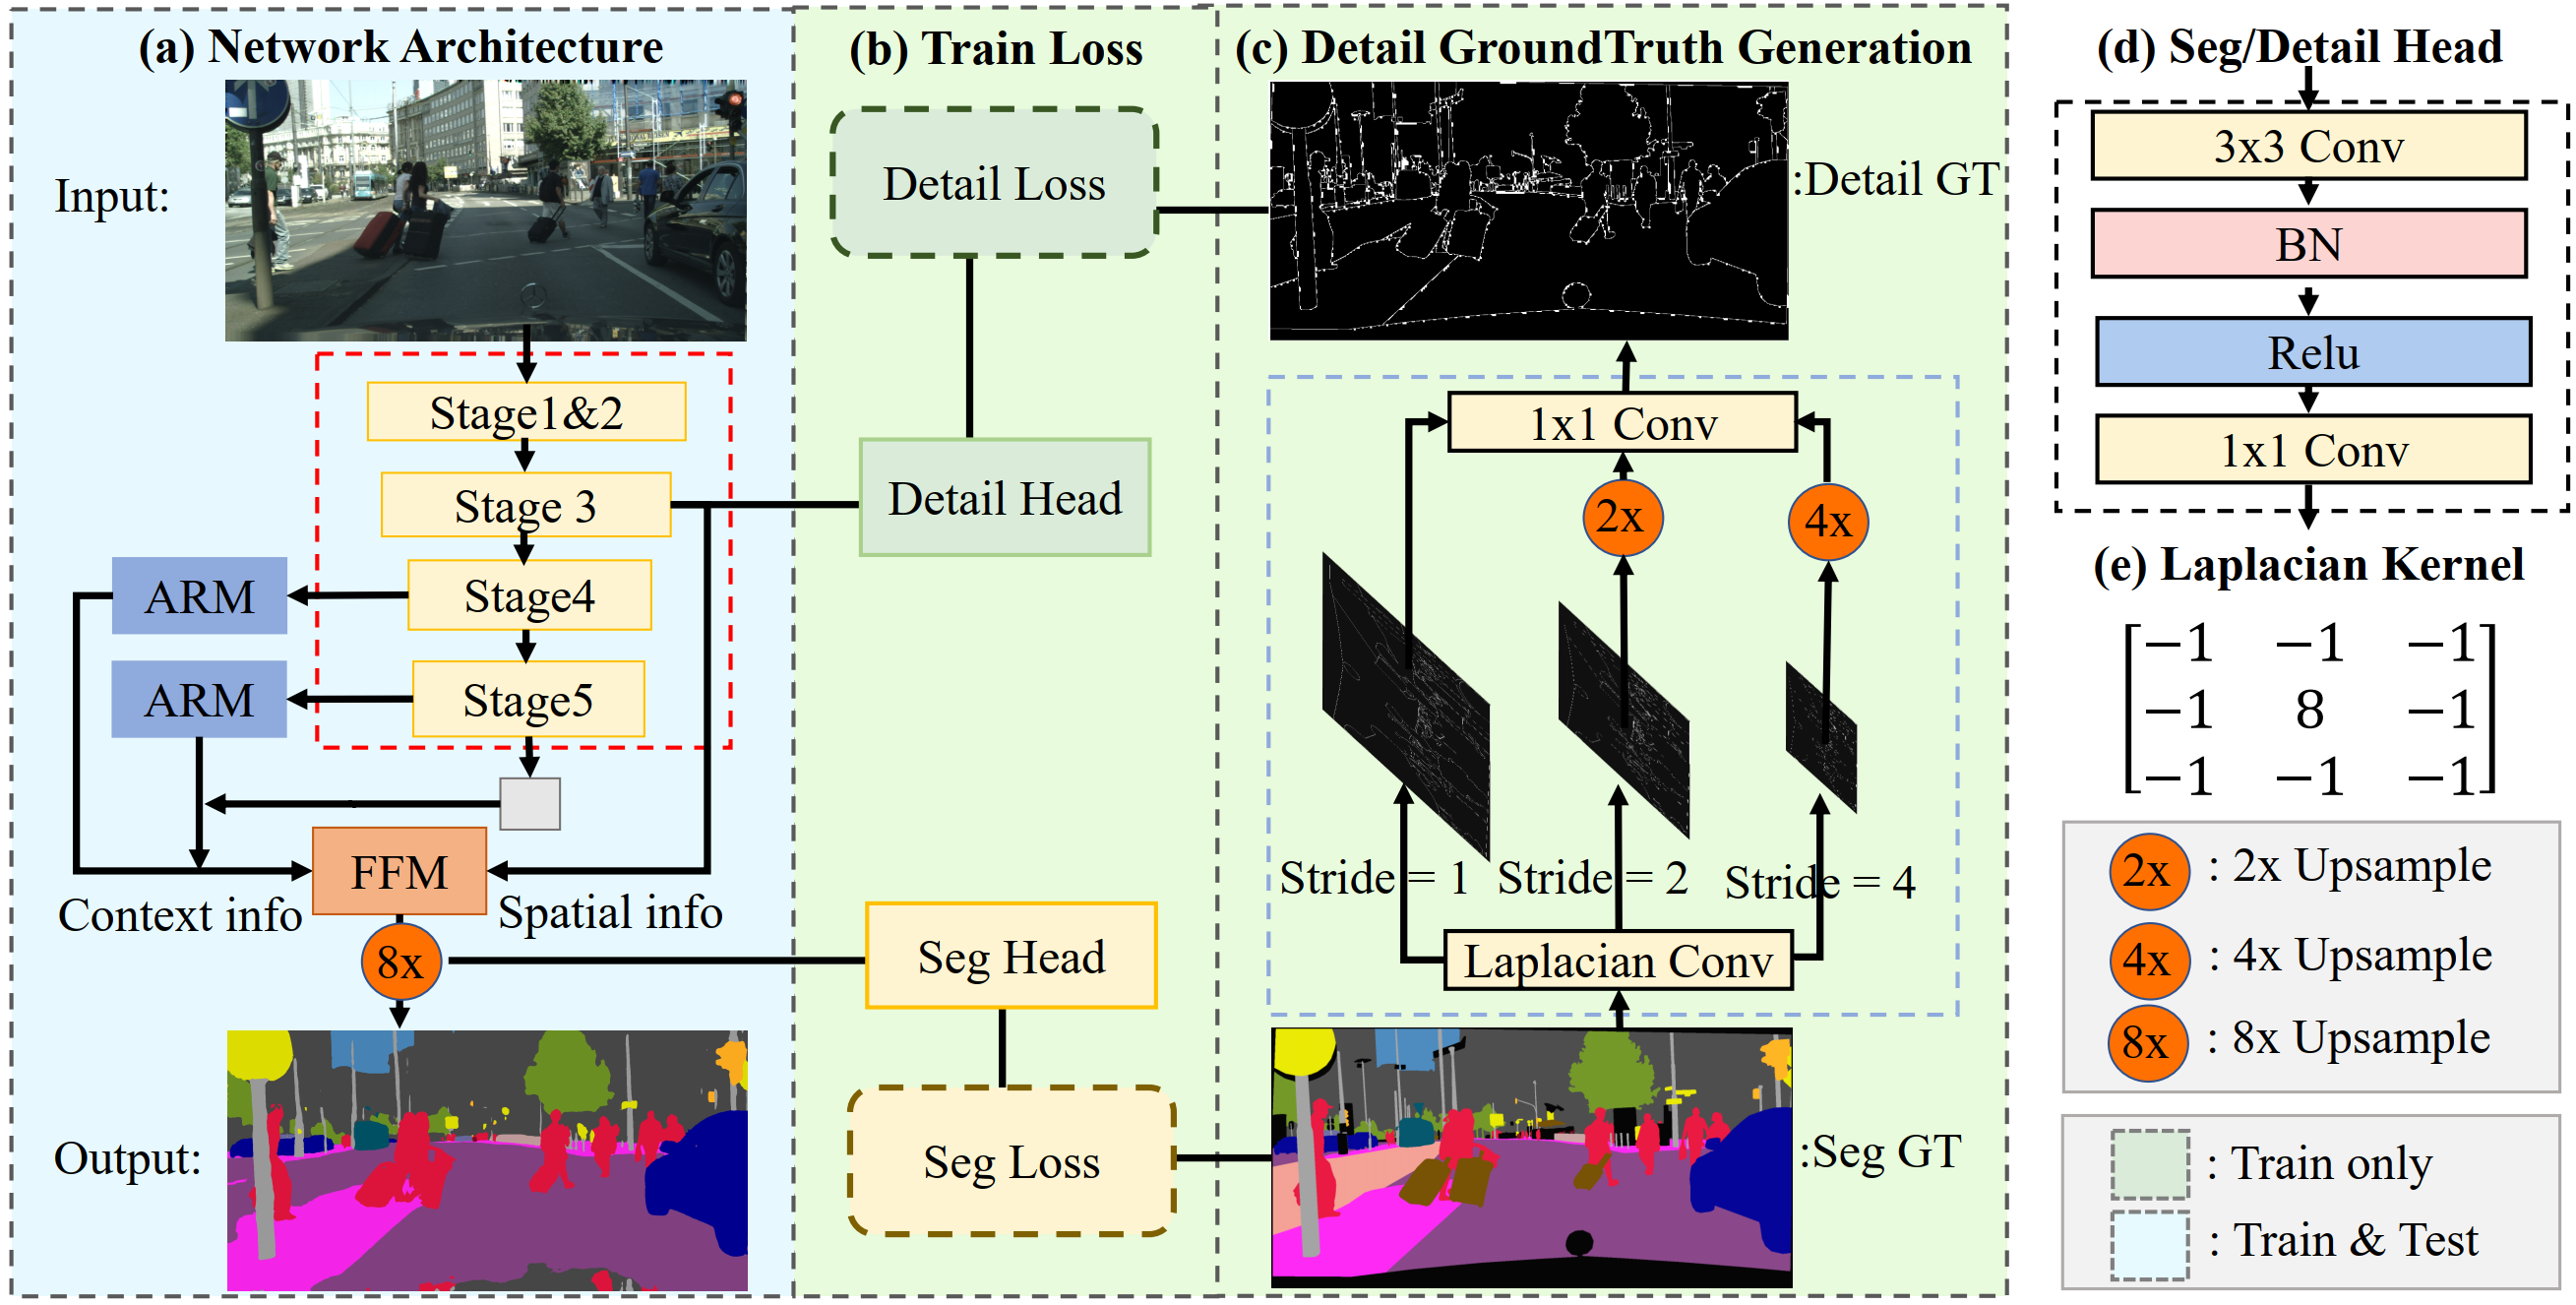
\includegraphics[width=1\linewidth]{img/stdcseg-architecture}
	\caption{Arquitetura completa da rede neural utilizada \cite{fan2021RethinkingBiSeNetRealtime}.}
	\label{fig:stdcseg-architecture}
\end{figure}


\subsection{\textit{Dataset} de treinamento e dados de teste}

Dataset... tamanho... particionamento... resolução... classes...

\subsection{Método de treinamento}

Batch... epocas... iterações...

\subsection{Métricas de avaliação}

mIOU50... mIOU75...

\subsection{Teste}

\section{Resultados}  \label{sc:resultados}

\begin{note}
	\begin{itemize}
		\item Para cada rede:
		\begin{itemize}
			\item Métricas 
			\item Segmentação
			\begin{itemize}
				\item Entrada
				\item \textit{Ground truth}
				\item Saída
			\end{itemize}
			\item Tempo de treinamento
		\end{itemize}
	\end{itemize}
\end{note}

\subsection{Métricas}

\subsection{Dados de teste}


\section{Análise dos Resultados}  \label{sc:analise}

\begin{note}
	\begin{itemize}
		\item Comparar as três redes:
		\begin{itemize}
			\item mIoU
			\item FPS
			\item Dados segmentados do \textit{dataset}
			\item Dados segmentados coletados no \textit{campus}
		\end{itemize}
		\item Apontar relação custo \textit{vs} desempenho de cada rede
		\item Considerar custos de treinamento
	\end{itemize}
\end{note}


\section{Conclusões}  \label{sc:conclusoes}

\begin{note}
	\begin{itemize}
		\item Retomar o problema inicial
		\item Destacar metodologia e os resultados que foram obtidos
		\item Comentar a análise dos resultados, mostrando que seria melhor para implementação
		\item Propor melhorias
		\item Propor validação de aplicação
		\item Listar proposta de aplicação dessa técnica
		\begin{itemize}
			\item Perception grid
		\end{itemize}
	\end{itemize}
\end{note}

\section*{Agradecimentos}

\begin{note}
	\begin{itemize}
		\item Levy e Romis
		\item Giovani?
	\end{itemize}
\end{note}

\section*{Referências}  \label{sc:referencias}

\nocite{geron2020HandsonMachineLearning}

\bibliographystyle{acm}
\renewcommand{\section}[2]{}
\bibliography{bibliograpy}

\end{document}